\documentclass{article}

\usepackage{amsmath, amssymb, amsthm}
\usepackage{geometry}
\geometry{verbose,tmargin=1cm,bmargin=2cm,lmargin=2cm,rmargin=2cm,marginpar=0cm}

\usepackage{tcolorbox}
\usepackage{fancyvrb}
\usepackage[hidelinks]{hyperref}
\usepackage{mathtools}
\usepackage{etoolbox}
\usepackage{enumitem}
\usepackage{stackrel}
\usepackage{multirow}
\usepackage{setspace}
\usepackage{arydshln}

\usepackage{graphicx} % Required for inserting images
\graphicspath{ {./Images/} }
\usepackage{stackengine,scalerel}
\usepackage[utf8]{inputenc}
\usepackage{babel}
\usepackage{dsfont}
\usepackage{listings}
\usepackage{multicol}
\usepackage{stmaryrd}
\usepackage{xcolor}
\usepackage{xurl}
\usepackage{titlesec}

\usepackage{fancyhdr}
\pagestyle{fancy}
\fancyhf{} 
\fancyfoot[L]{MATH3205 Report}
\fancyfoot[C]{Hugo Burton, Anna Henderson \& Mitchell Holt}
\fancyfoot[R]{\thepage}
\renewcommand{\headrulewidth}{0pt} % Remove the line at the top of the page
\renewcommand{\footrulewidth}{0.4pt} % Add a line just above the footer

\setstretch{1.2}

\newcommand{\E}{\mathcal{E}}
\newcommand{\scriptP}{\mathcal{P}}
\newcommand{\scriptR}{\mathcal{R}}
\newcommand{\scriptK}{\mathcal{K}}
\newcommand{\scriptE}{\mathcal{E}}
\newcommand{\B}{\mathbb{B}}
\newcommand{\Z}{\mathbb{Z}}

\newcommand{\set}[1]{%
  \left( #1 \right)
}

\newcommand{\inlinecode}[1]{\colorbox{gray!20}{\texttt{#1}}}

\setlength{\parindent}{0pt}

\title{MATH3205 - Report}
\author{Hugo Burton, Anna Henderson and Mitchell Holt}

\begin{document}
\maketitle

\thispagestyle{fancy}

\tableofcontents


\newpage

\section{Problem Description}
\subsection{Approaches}
The source paper entitled \textit{``Exact and metaheuristic methods for real-world examination timetabling problem"} was published in the Journal of Scheduling in May of 2023. This paper investigated optimising Italian university examination schedules by meeting a set of hard constraints, and minimising what they referred to as soft constraints, or more descriptively, penalty terms. To summarise, university courses had one or more examinations, and each examination could be either written, oral, or contain both parts, which were referred to as \textbf{Events}. These courses were organised into primary and secondary curricula, with primary courses being more commonly enrolled, as enrollment figures were unknown at the time of solving the problem. \medbreak

The penalty terms can be split into the three main types; conflicts, preferences and distances. Conflicts occur when events belong to the same curriculum, either as primary-primary, or primary-secondary, scheduled in the same time period would impose a penalty. Preferences can occur for periods, event-periods, event-rooms or room-periods and have been summarised in the following table

\begin{table}[htb]
    \centering
    \begin{tabular}{|l|l|}
        \hline
        \textbf{Preference Name} & \textbf{Possible Levels} \\
        \hline
        Period & Undesired \\ \hdashline
        \multirow{2}{*}{Event-Period} & Undesired \\
                                     & Preferred \\ \hdashline
        Event-Room & Undesired \\ \hdashline
        Room-Period & Undesired \\
        \hline
    \end{tabular}
    \caption{Types of Preferences}
    \label{tab:preferences_types}
\end{table}

Finally, penalties are imposed when two events do not meet a distance constraint, either directed or undirected. Directed meaning that the first event (in the tuple) must precede the latter, and undirected meaning a minimum distance must exist between the events. Directed distance constraints occur when
\begin{enumerate}
    \item an Examination has a written and oral event, with written always preceding the oral component.
    \item there are multiple examinations for one course, each with an ordinal index: the examination's respective events must occur in order of the exam ordinal index. (In cases where the examination is written and oral, only the first, written, event component needs to be in order.
\end{enumerate}

Undirected distance constraints occur when
\begin{enumerate}
    \item Two courses belong to the same curriculum, with varying penalty weights depending upon the curriculum the pair of events is from.
\end{enumerate}

It is also important to note that some periods and rooms may also be forbidden for certain events or for all events in individual periods, which, if broken, result in an infeasible solution.
\bigbreak

\subsubsection*{Methods Explored}
The paper explored a variety of approaches to try to solve this problem including a MIP (via both Gurobi 9.1.0 and MiniZinc), Simulated Annealing, and Constraint Programming. A two stage decomposition was briefly mentioned, and results were actually given, however, the formulation wasn't made explicit. That is, some constraints were given, but they mentioned that their constraints weren't ideal. The proposed two stage decomposition stipulated that events first be assigned to periods in a master problem, followed by events being assigned to rooms in the second stage or sub-problem. For this to be successful we need to ensure that the solution found in the initial stage can be easily fixed in the event that the sub-problem proves to be infeasible, e.g. due to a lack of compatible rooms. \medbreak

The constraint programming formulation in the paper utilised a heuristic search method as they discovered that the exhaustive search is not effective for this problem. The heuristic search used large neighbourhood search and restarts on top of a branch and bound scheme. Within the MIP model, the paper actually found that using MiniZinc was superior to Gurobi due to it's better support for binary multiple value domains and linearising constraints. Finally the simulated annealing approach considered two vectors which were used to represent a state in the search space where the period and rooms for each event were stored. Having said that, for our formulation, the Gurobi solver (v10.0.3) was implemented in Python.

\bigbreak

\subsection{Results}
After implementing firstly the Naive implementation from the paper, and then modifying this as per the formulation below in section \ref{benders_formulation}, the following results were achieved. Note that runtime was capped at 1 hour per problem set for the paper's implementation while we set a limit of 30 minutes as for all the problem sets, little progress was made after this time. Despite our best efforts, we found that many of the problem sets were simply too computationally difficult to solve exactly with the hardware we had. \medbreak

The paper itself found the best solution with their MIP implementation, while the simulated annealing, and CP approach often did not achieve the exact objective. As per the results in Table 8 of the original paper, the simulated annealing approach was often slightly above the MIP, while the CP implementation proved far inferior. \medbreak

The paper was able to utilise server hardware with 756GB RAM and 2x Intel Xeon Gold 6226R CPUs @ 2.90GHz. While our setup arguably had a faster CPU (at least single threaded performance which is more optimal for Gurobi) with a Core i7-12700K @ 5GHz, we were limited by memory with only 32 GB DDR5 @ 5200 MHz. Testing found that many of the large problem sets had too many nodes to store in this much memory which slowed down computation significantly.

\begin{table}[htb]
    \centering
    \begin{tabular}{|l|r|r|}
        \hline
        \textbf{Problem Set} & \textbf{Our Objective (Benders)} & \textbf{Paper's Objective} \\
        \hline
        D1-1-16 & 544 & 381 \\
        D1-1-17 & 424 & 318 \\
        D1-2-16 & 652 & 521 \\
        D1-2-17 & 856 & 609 \\
        D1-3-16 & 1000 & 720 \\
        D1-3-17 & 854 & 612 \\
        D1-3-18 & 304 & 264 \\
        D2-1-18 & 892 & 426 \\
        D2-2-18 & 34 & 22 \\
        D2-3-18 & 34 & 22 \\
        D3-1-16 & 8 & 0 \\
        D3-1-17 & 15 & 0 \\  
        D3-1-18 & 828 & 0 \\
        D3-2-16 & 2 & 0 \\
        D3-2-17 & 0 & 0 \\
        D3-3-16 & 0 & 0 \\
        D3-3-17 & 0 & 0 \\
        D3-3-18 & 30 & 0 \\
        D4-1-17 & 280 & 276 \\
        D4-1-18 & 1690 & 1028 \\
        D4-2-17 & 2132 & 1105 \\
        D4-2-18 & 2903 & 1579 \\
        \hline
    \end{tabular}
    \caption{Comparison of our objective value and the paper's objective value}
    \label{tab:comparison}
\end{table}


\begin{table}[htb]
    \centering
    \begin{tabular}{|l|r|r|}
        \hline
        \textbf{Problem Set} & \textbf{Our Objective (Benders)} & \textbf{Paper's Objective} \\
        \hline
        D4-3-17 & 442 & 372 \\
        D4-3-18 & 907 & 670 \\
        D5-1-17 & 328 & 156 \\
        D5-1-18 & 84 & 36 \\
        D5-2-17 & 120 & 60 \\
        D5-2-18 & 688 & 264 \\
        D5-3-18 & 0 & 0 \\
        D6-1-16 & 1146 & 432 \\
        D6-1-17 & 879 & 360 \\
        D6-1-18 & 1100 & 392 \\
        D6-2-16 & 945 & 506 \\
        D6-2-17 & 1459 & 558 \\
        D6-2-18 & 383 & 199 \\
        D6-3-16 & 128 & 27 \\
        D6-3-17 & 137 & 30 \\
        D7-2-17 & 1648 & 758 \\
        toy & 2 & 0 \\
        \hline
    \end{tabular}
    \caption{Comparison of our objective value and the paper's objective value}
    \label{tab:comparison_@}
\end{table}

\newpage

\section{Insight}
\subsection{Structure, Scale and Initial Approach}\label{ref:structure_scale_approach}

While assigning university examinations to periods and rooms may not seem at at first too difficult to solve, this particular problem includes many intricacies which do indeed complicate the structure of the MIP formulation greatly. This problem is complicated primarily for two main reasons. Firstly, there are many highly specific constraints (i.e. the penality terms) which require certain sets to be generated prior to defining the model. Secondly, the configuration of rooms with both types and number of joining rooms, as well as rules about compatible rooms further adds to the complexity in setting up the structure of the implementation. \\
\\
In an effort to reduce error and improve efficiency, knowing that the difficulty would only increase with Bender's decomposition, we considered each part of the formulation systematically. Firstly the structure of each object in the problem was designed: e.g. Courses, Exams, Events, Curriculas, ..., etc. In doing so, creating all the sets for each part of the problem could be approached independently, which made it easier working in a team. Additionally, this approach made for smaller concepts that are easier to maintain, should the formulation of the problem ever be adapted. \\
\\
With all the sets defined, approaching the naive formulation was simple as this was given in the paper, though it was found the paper was light on details about the sets and variables in some places meaning that some knowledge and understanding of the problem wasn't discovered until the time of implementation. \\
\\
Such a modular approach to our formation allows for this problem to be scaled, not only to larger data sets, but also generalised to similar problems. For example, examination schedules at other universities may have both differing penalty conditions, or even a different structure of courses and their examinations. 

\newpage

\subsection{Difficulty in Implementing the Naive Formulation}

To implement the naive formulation of the problem we first created an object oriented \texttt{Python} code base, containing custom classes and some helper methods to read the instance \texttt{json} data from the paper, and convert this into sets used by Gurobi. As mentioned in section \ref{ref:structure_scale_approach}, each object in the problem was segmented into it's own Python module, which allowed for easy, independent development of each part of the program - the modules are listed below.
\setlist[enumerate]{itemsep=2pt}
\begin{enumerate}
    \item \inlinecode{Constants.py} - constants file
    \item \inlinecode{Utils.py} - Extra helper functions
    \item \inlinecode{Course.py}
    \begin{enumerate}
        \item \inlinecode{CourseManager} - stores all the Courses in the problem set
        \item \inlinecode{Course} - a course object
        \item \inlinecode{RoomsRequested} - stores the data for rooms requested by a course's events
        \item \inlinecode{WrittenOralSpecs} - stores data about the events when a course has exams of both written and oral components.
    \end{enumerate}
    \item \inlinecode{Examination.py} - derived from courses and contains written, oral or both written and oral events.
    \item \inlinecode{Event.py} - derived from examinations and has type written or oral
    \item \inlinecode{Curriculum.py}
    \begin{enumerate}
        \item \inlinecode{Curriculum} - stores a single Curriculum within the set of Curriculas in the problem set.
        \item \inlinecode{CurriculaManager} - stores all the curriculas for the problem set
    \end{enumerate}
    \item \inlinecode{Room.py}
    \begin{enumerate}
        \item \inlinecode{Room} - stores a room object, either composite or single
        \item \inlinecode{RoomManager} - stores all the rooms on campus for the problem set
    \end{enumerate}
    \item \inlinecode{Period.py}
    \item \inlinecode{Constraint.py}
    \begin{enumerate}
        \item \inlinecode{Constraint} - Abstract Class of Generic Constraint in the problem set
        \item \inlinecode{RoomPeriodConstraint} - Constraints involving rooms and periods
        \item \inlinecode{EventPeriodConstraint} - Constraints involving Events and Periods
        \item \inlinecode{EventRoomConstraint} - Constriants involving Events and Rooms
        \item \inlinecode{PeriodConstraint} - Constraints involving Periods only
        \item \inlinecode{ConstraintManager} - stores all the constraints from the problem set.
    \end{enumerate}
\end{enumerate}

Implementing the initial approach took much longer than anticipated, due to the many constraints and custom sets that had to be derived from the data. In an effort to keep the main script, \inlinecode{BendersImplementationAllTricks.py}, as small as possible, much of the code specific to each of the above objects in the problem was abstracted away in each module. Having said that, $\sim 600$ lines of the solve function is dedicated just to generating the sets. As a result of this complexity and lack of documentation in the original paper, some bug were discovered only at the time of implementing Bender's decomposition, which slowed the development process. For example, it was not realised that events could have preferred periods as well as undesired and forbidden until this time. In future projects, a more thorough breakdown of the problem, perhaps as a mindmap, would be a good idea to ensure small details do not go unmissed. \\
\\
In order to determine the accuracy of our solutions against the solutions from paper, we also attempted to implement a cost finder program, found in \inlinecode{FindCosts.py}, which gets the solution file from the paper and calculates the contribution of each of the penalty soft constraints to the objective. The hopes of this function was to allow us to determine which soft constraints we are over or under calculating and allow us to debug our implementations. Unfortunately, although the function is able to calculate the majority of the costs, we were unable to get it fully functioning due to the large number of edge cases that needed to be considered. \\
\\
Some other small modules were written including
\begin{enumerate}
    \item \inlinecode{ProblemSets.py} which gets all the objectives from both our solutions and the paper's then converts this into a Latex table.
    \item \inlinecode{SolutionExport.py} which is called upon in the main script to save our model's variable outputs into the same \texttt{json} format that the paper gave their solutions in. 
\end{enumerate}


\subsection{Implementing the Proposed Improvements}
The initial work of implementing the Naive solution was arguably the most difficult part of this project. Modifying it to work with Bender's decomposition did, however, require significant thought and much fine tuning of parameters in order to achieve optimal performance. Our implementation of Benders Decomposition involved a two-part disaggregation to assign periods to events in the master problem, and then events to rooms in the sub problem. We began by separating the rooms dimension out from the existing formulation. This meant modifying the $x_{e, p, r}$ variable from the master (existing) formulation, and moving it into the sub-problem. As each sub-problem corresponded to one period, the $p$ dimension was dropped, leaving $x_{e, r} \forall e \in \E_p, r \in R_e$ as the only variable in the sub-problem where $\E_p$ is now defined as the events turned on by the master problem in period $p$. \\
\\
Then, any constraints involving $x$ were moved into the sub-problem - primarily these were constraints around ensuring one event per room, and one room per event, etc. The one constraint which linked $y$ to $x$ was discarded, as this was now made implicit within the construction of the sub-problem. Initially, the decomposition was implemented within a \inlinecode{while} loop where the master problem was solved, before the each of the $P$ sub-problems, however, due to the master problem being significantly more difficult, this was built into a \texttt{callback} function early on in development. \\
\\
Finally, the optimality and feasibility cuts were added to the sub-problem which completed the development of the Bender's Implementation. \\
\\
Some time was also spent tuning the parameters for Gurobi in an effort to push the limit of performance. The following parameters were settled upon as best:

\begin{table}[htb]
    \centering
    \begin{tabular}{|l|r|}
        \hline
        \textbf{Gurobi Hyperparameter} & \textbf{Value} \\
        \hline
        MIPGap & 0 \\
        LazyConstraints & 1 \\
        Presolve & 2 \\
        MIPFocus & 2 \\
        TimeLimit & $60 \times 60$ (seconds) \\
        SoftMemLimit & 60 (GB) \\
        \hline
    \end{tabular}
    \caption{Gurobi Hyperparamter Values}
    \label{tab:gurobi_param_values}
\end{table}

\newpage
It was found that setting presolve to aggressive mode did improve the solution slightly for the same runtime as leaving this default. Even though the time for presolve took longer, this was still no more than 20 seconds even for large problems, which isn't significantly longer than a standard presolve. Additionally, the reasoning behind setting \texttt{MIPFocus} to $2$ was that the model was having no trouble finding feasible solutions, even for problem sets with lots of composite rooms. This means that more effort can be put towards proving optimality. While a \texttt{MIPFocus} of $3$ was tested, this didn't seem to improve performance from a setting of $2$.\\
\\
The initial paper applied a time limit constraint of 1 hr to all of the data instances. This resulted in some instances reaching optimality and others returning the best found solution at the conclusion of the 1 hr time limit. Whilst testing our Benders formulation, the \texttt{TimeLimit} was set to 30 minutes to try and achieve a reasonable solution for every instance, rather than to reach optimality. However, for our final implementation we chose to match the paper and ultimately settled on a \texttt{TimeLimit} of 1 hour.

\newpage

\section{Naive Formulation}
This section describes the direct MIP formulation given in the paper, which was the main
focus of our attention. We implemented this model ourselves and tested the performance of
our own implementation against it.
\subsection{Sets}

\begin{itemize}
    \item $\scriptE$ - set of events
    \item $\scriptP$ - set of periods
    \item $\scriptR$ - set of rooms
    \item $\scriptR^c$ - set of composite rooms $(\scriptR^c \subset \scriptR)$
    \item $\scriptR^0_{r^c}$ - set of overlapping rooms of composite rooms
    \item $\scriptP_e$ - set of available periods for event $e$
    \item $\scriptR_e$ - set of available rooms for event $e$
    \item $F$ - set of examination pairs with (hard) precedence constraints
    \item $HC_e$ - set of events in hard conflict with $e\in \scriptE$
    \item $DP^{\leftarrow}$ - set of event pairs with directed soft distance constraint
    \item $DP^{\leftrightarrow}$ - set of event pairs with undirected soft distance constraint
    \item $O(\cdot)$ - ordinal number of a period
    \item $DP^{E}$ - set of exams of the same course
    \item $DP^{WO}$ - set of written and oral events of the same examination
    \item $DP^{\leftarrow}$ - set of pairs of events having a soft distance constraint where $e_1$ ideally comes before $e_2$.
    \item $DP^{\leftrightarrow}$ - set of pairs of events where $e_1$ has a soft undirected distance constraint from $e_2$
    \item $DP^{PP}$ - set of pairs of events existing in the same primary curriculum. Only applies to the first examinatoin if there are multiple exams for the one course.
    \item $DP^{PS}$ - set of pairs of events in at least 1 secondary curriculum.    
    \item $SC^{PS}_e$ - set of secondary events in the same curriculum as the primary event $e$
    \item $SC^{SS}_e$ - set of secondary events (not including itself) in the same curriculum as the secondary event $e$
\end{itemize}

\bigbreak

\subsection{Variables}

$X_{e,p,r} \in \B$ - 1 if event $e$ assigned to period $p$ and room $r$

$Y_{e,p} \in \B$ - 1 if event $e$ assigned to period $p$

$h_e\in \Z_0$ - ordinal value of the period assigned to event e

$d_{e_1, e_2} \in \Z_+$ - the absolute distance value between assignments of $e_1$ and $e_2$
$d^{\leftrightarrow}_{e_1, e_2} \in \Z$ - the actual distance value between assignments of $e_1$ and $e_2$

$g^{\leftrightarrow}_{e_1, e_2} \in \B$ - 1 if $d^{\leftrightarrow}_{e_1, e_2}$ is positive

$d^{abs_1}_{e_1, e_2}\in \Z_+$ - the absolute value of $d^{\leftrightarrow}_{e_1, e_2}$ or zero.
$d^{abs_2}_{e_1, e_2}\in \Z_+$ - the absolute value of $d^{\leftrightarrow}_{e_1, e_2}$ or zero.

$p^{\min E}_{e_1, e_2}$ - 1 if $e_1$ and $e_2$ are events within the same examination

\bigbreak

\subsection{Constraints}

\begin{align}
    \sum_{p\in\scriptP_e}\sum_{r\in\scriptR_e} x_{e,p,r} &= 1 \forall e \in \scriptE \\
    \sum_{e\in \scriptE} x_{e,p,r} &\le 1 \forall r \in \scriptR p \in \scriptP \\
    |\scriptR^0_{r^c}| \sum_{e\in\scriptE} x_{e,p,r} + \sum_{r_0\in\scriptR^0_{r^c}}\sum_{e\in \scriptE}x_{e,p,r^0} &\le |\scriptR^0_{r^c}| \forall r^c \in \scriptR^c, \forall p \in \scriptP \\
    h_{e_1} - h_{e_2} &\le -1 \forall(e1, e2) \in F \\
    |HC_{e}| \cdot Y_{e,p} + \sum_{e2 \in HC_e}y_{e2, p} &\le |HC_{e}| \forall e\in \scriptE, p \in P_{e} \\
    y_{e,p} - \sum_{r\in\scriptR} x_{e,p,r} &= 0 \forall e \in \scriptE, p \in \scriptP_e \\
    \sum_{p\in \scriptP_e}O(p) \cdot y_{e,p} &= h_{e} \forall e \in \scriptE \\
\end{align}

\subsubsection{Soft (penalty) Constraints}

\begin{align}
    &|\{e_2 \in SC_e^{PS}: O(e) < O(e_2) ^ p \in P_{e_2}\}| y_{e,p} \nonumber \\
    &+ \sum_{e_2 \in SC^{PS}_e : O(e) < O(e_2)} y_{e_2, p} \nonumber\\
    &\le s^{PS}_{e,p} + |\{e_2 \in SC_e^{PS}: O(e) < O(e_2) ^ p \in P_{e_2}\}| \forall e \in \scriptE, p \in \scriptP_e \\
    &|\{e_2 \in SC_e^{SS}: O(e) < O(e_2) ^ p \in P_{e_2}\}| y_{e,p} \nonumber\\ 
    &+ \sum_{e_2\in SC_e^{SS}:O(e)<O(e_2)} y_{e_2, p} \nonumber\\
    &\le e^{SS}_{e,p} + |\{e_2 \in SC_e^{SS}: O(e) < O(e_2) ^ p \in P_{e_2}\}|, \forall e \in \scriptE, p \in \scriptP_e \\
    d_{e_1, e_2} &= h_{e_2} - h_{e_1}, \forall (e1, e2) \in DP^{\leftarrow}
\end{align}

\begin{align}
    d^{\leftrightarrow}_{e_1, e_2} &= h_{e_2} - h_{e_1}  , \forall (e1, e2) \in DP^{\leftrightarrow} \\
    d^{\leftrightarrow}_{e_1, e_2} &\le |\scriptP|\cdot g^{\leftrightarrow}_{e_1, e_2}  , \forall (e1, e2) \in DP^{\leftrightarrow} \\
    d^{\leftrightarrow}_{e_1, e_2} &\ge - |\scriptP| (1 - g^{\leftrightarrow}_{e_1, e_2})   , \forall (e1, e2) \in DP^{\leftrightarrow} \\
    d^{abs_1}_{e_1, e_2} &\le |\scriptP|g^{\leftrightarrow}_{e_1, e_2}  , \forall (e1, e2) \in DP^{\leftrightarrow} \\
    d^{abs_1}_{e_1, e_2} &\ge - |\scriptP|g^{\leftrightarrow}_{e_1, e_2}  , \forall (e1, e2) \in DP^{\leftrightarrow} \\
    d^{abs_1}_{e_1, e_2} &\le d^{\leftrightarrow}_{e_1, e_2} + |\scriptP| (1 - g^{\leftrightarrow}_{e_1, e_2}  , \forall (e1, e2) \in DP^{\leftrightarrow} \\
    d^{abs_1}_{e_1, e_2} &\ge d^{\leftrightarrow}_{e_1, e_2} - |\scriptP| (1 - g^{\leftrightarrow}_{e_1, e_2}  , \forall (e1, e2) \in DP^{\leftrightarrow} \\
    d^{abs_2}_{e_1, e_2} &= d^{abs_1}_{e_1, e_2} - d^{\leftrightarrow}_{e_1, e_2}  , \forall (e1, e2) \in DP^{\leftrightarrow} \\
    d_{e_1, e_2} &= d^{abs_1}_{e_1, e_2} + d^{abs_2}_{e_1, e_2} , \forall (e1, e2) \in DP^{\leftrightarrow} 
\end{align}

\begin{align}
    p^{\min E}_{e_1, e_2} + d_{e_1, e_2} &\ge P^{min}_{e_1, e_2}, \forall (e_1, e_2)\in DP^{E} \\
    p^{\min WO}_{e_1, e_2} + d_{e_1, e_2} &\ge P^{min}_{e_1, e_2}, \forall (e_1, e_2)\in DP^{WO} \\
    d_{e_1, e_2} - p^{\max WO}_{e_1, e_2} &\le P^{max}_{e_1, e_2}, \forall (e_1, e_2)\in DP^{WO} \\
    p^{\min PP}_{e_1, e_2} + d_{e_1, e_2} &\ge P^{min}_{e_1, e_2}, \forall (e_1, e_2)\in DP^{PP} \\
    p^{\min PS}_{e_1, e_2} + d_{e_1, e_2} &\ge P^{min}_{e_1, e_2}, \forall (e_1, e_2)\in DP^{PS}
\end{align}

\bigbreak

\subsection{Objective Function}

\begin{align} 
    \min &\beta^{PS}\sum_{e\in \scriptE}\sum_{p\in\scriptP_e}s^{PS}_{e,p} + \beta^{SS}\sum_{e\in\scriptE}\sum_{p\in\scriptP_e}s^{SS}_{e,p} \nonumber \\
    &+\sum_{e\in\scriptE}\sum_{p\in\scriptP_e}\alpha_{ep}y_{e,p} \nonumber \\
    &+\sum_{e\in\scriptE}\sum_{p\in\scriptP_e}\sum_{r\in\scriptR_e}\alpha_{er}x_{e,p,r}
    + \gamma^E\sum_{(e1, e2)\in DP^{E}} p^{\min E}_{e_1, e_2} \nonumber \\
    &+ \gamma^{WO} \sum_{(e1, e2)\in DP^{WO}}\left(p^{\min WO}_{e_1, e_2} + p^{\max WO}_{e_1, e_2}\right) \nonumber \\
    &+ \gamma^{PP}\sum_{(e_1, e_2)\in DP^{PP}} p^{\min PP}_{e_1, e_2)}
    + \gamma^{PS}\sum_{(e_1, e_2)\in DP^{PS}} p^{\min PS}_{e_1, e_2)}
\end{align}

\newpage

\section{Benders Formulation}\label{benders_formulation}
Our formulation of the problem uses Benders' decomposition.

\subsection{Master Problem (BMP)}
The master problem will assign events to time periods (with no consideration of
how events will be assigned to rooms within each time period).

\subsubsection*{Sets}
\begin{itemize}
    \item $\E$ the set of events
    \item $P$ the set of periods, each of which is assigned an ordinal value
        $0,1,\dots, |P| - 1$.
    \item $PA_e \subseteq P$ the set of available periods for event $e \in \E$
    \item $PD \subseteq E$ the set of all events with period preferences.
    \item $PU \subseteq E$ the set of all events with undesired periods.
    \item $PB \subseteq P$ the set of all periods which are undesired (for all
        events).
    \item $P1$ the set of all unordered pairs $s$ of events $s = \{e_1, e_2\}$
        for which there exists a curriculum with courses $c_1 \neq c_2$, not
        both primary courses, such that $e_1$ and $e_2$ are examination events
        for $c_1$ and $c_2$ respectively.
    \item $P2 \subseteq \E$ the set of all events which have undesired rooms.
    \item $C$ the set of curricula.
    \item $T$ the set of teachers.
    \item $F \subset \E \times \E$ the set of pairs of events where the first
        event must precede (that is, be scheduled strictly before) the second.
        An event $e_1$ must precede an event $e_2 \in \E$ if they are consecutive
        parts of the same examination, or if they belong to consecutive
        examinations of the same course.
    \item $DP^\leftarrow$ and $DP^\leftrightarrow$ the sets of pairs of events
        with desired undirected or directed separations respectively.
    \item $DP^E$ the set of pairs of events belonging to examinations of the same
        course.
    \item $DP^{WO}$ the set of pairs of written/oral events of the same examination.
    \item $DP^{PP}$ the set of pairs of events which correspond to courses which are
        both primary for some curriculum.
    \item $DP^{PS}$ the set of pairs of events which correspond to courses which are
        primary and secondary respectively for some curriculum. 
\end{itemize}

\subsubsection*{Data}
\begin{itemize}
    \item $O_p \in \{0,1,\dots,|P| - 1\}$ the ordinal value of the period $p \in
        P$.
    \item $RA_e$ the set of rooms to which the event $e \in \E$ could be
        assigned.
    \item $PA_e$ the set of periods to which the event $e \in \E$ could be
        assigned.
    \item SOFT\_CONFLICT$_s$ the $S1$ penalty for the unordered event pair $s \in
        P1$.
    \item UNDESIRED\_PERIOD the fixed penalty for assigning an event $e \in PU$
        to an undesired period.
    \item NOT\_PREFERRED the fixed penalty for assigning an event $e \in PD$ to
        a period other than that which is preferred.
    \item UNDESIRED\_ROOM the fixed penalty for assigning an event $e \in P2$ to
        an undesired room.
    \item $UP_e$ the set of undesired periods for $e \in PU$.
    \item $PP_e$ the set of preferred periods for $e \in PD$.
    \item $UR_e \subset RA_e$ the set of undesired rooms for $e \in P2$.
    \item $R_p$ the set of rooms available in the period $p \in P$.
    \item $C^P_c$ the set of events belonging to primary courses of curriculum
        $c \in C$.
    \item $C^T_t$ the set of events belonging to courses taught by teacher $t
        \in T$.
    \item $P_{e_1, e_2}^\text{min}, P_{e_1, e_2}^\text{max}$ the respective
        minimum/maximum preferred distances between the events $e_1, e_2 \in
        DP^\leftarrow \cup DP^\leftrightarrow$.
    \item $\gamma^{TYPE}$ the distance penalty cost for events in $DP^{TYPE}$, where
        type is one of $E$, $WO$, $PP$ or $PS$.
\end{itemize}

\bigbreak

\subsubsection*{Variables}
\begin{itemize}
    \item $y_{e, p} \in \{0,1\}$ the decision variable assigning events $e$ to
        periods $p \in PA_e$.
    \item $S1_s$ the penalty for a soft conflict between the events in the
        unordered pair events $s$, for all $s \in P1$. Although these variables
        must have integer values, they may be relaxed to be continuous as they
        will naturally attain integer values (see constraint \eqref{setS1}).
    \item $S2_p$ the estimate of the number of events allocated to undesired
        rooms in period $p \in P$. These variables may also be relaxed to be
        continuous.
    \item $h_e$ the ordinal value of the period to which the event $e \in \E$ is
        scheduled.
    \item $d_{e1, e2}$ the distance between the events $e_1, e_2 \in
        DP^{\leftarrow} \cup DP^{\leftrightarrow}$.
    \item $p_{e_1, e_2}^{minE}$ the variable counting the penalty for violating
        the minimum distance between the events $e_1, e_2 \in DP^E$.
    \item $p_{e_1, e_2}^{minWO}$ the variable counting the penalty for violating
        the minimum distance between the events $e_1, e_2 \in DP^{WO}$.
    \item $p_{e_1, e_2}^{maxWO}$ the variable counting the penalty for violating
        the maximum distance between the events $e_1, e_2 \in DP^{WO}$.
    \item $p_{e_1, e_2}^{minPP}$ the variable counting the penalty for violating
        the minimum distance between the events $e_1, e_2 \in DP^{PP}$.
    \item $p_{e_1, e_2}^{minPS}$ the variable counting the penalty for violating
        the minimum distance between the events $e_1, e_2 \in DP^{PS}$.
\end{itemize}

\subsubsection*{Objective}
\begin{multline}
    \min \quad \sum_{s \in P1} S1_s \quad + \quad \text{UNDESIRED\_PERIOD}
        \left( \sum_{e \in \E} \ \sum_{p \in PB \cap PA_e} y_{e, p} +
        \sum_{e \in PU} \sum_{p \in UP_e} y_{e, p} \right) \\
    + \quad \text{NOT\_PREFERRED} \sum_{e \in PD} \sum_{p \in PP_e} (1 - y_{ep})
        \quad + \quad \text{UNDESIRED\_ROOM} \sum_{p \in P} S2_p \quad + \quad
        \sum_{s \in P3} S3_s \\
    +  \gamma^E \sum_{s \in DP^E} p_s^{minE}  +  \gamma^{WO}
        \sum_{s \in DP^{WO}} \left(p_s^{minWO} + p_s^{maxWO}\right)  +
         \gamma^{PP} \sum_{s \in DP^{PP}} p_s^{minPP}  + 
        \gamma^{PS} \sum_{s \in DP^{PS}} p_s^{minPS}
\end{multline}

\subsubsection*{Constraints}
Each event must be scheduled to exactly one time period (BSP in \S\ref{BSP} will
allocate events to rooms once the period assignment has been fixed here):
\begin{equation}
    \sum_{p \in P \; : \; p \in PA_e} y_{e,p} = 1 \qquad \forall e \in \E
\end{equation}

We need to make sure that $S1$ is exactly the penalty for a soft conflict (two
events from a common curriculum being scheduled at the same time). To do this,
we will ensure that $S1_s \geq 0$ (which can be implemented by setting the lower
bound for the variable in the Gurboi API) and that it achieves the cost if and
only if two events are in soft conflict:
\begin{gather} \label{setS1}
    S1_{\{e_1, e_2\}} \geq \text{SOFT\_CONFLICT}_{\{e_1, e_2\}}
        (y_{e_1, p} + y_{e_2, p} - 1) \qquad \forall \{e_1, e_2\} \in P1, \
        \forall p \in PA_{e_1} \cap PA_{e_2}
\end{gather}

We will set the values of the $h$ with variables and use them to enforce
precedences with \eqref{seth} and \eqref{prec} below. Notice that we can
actually express these constraints equivalently (and more efficiently) without
introducing $h$, but the existence of this variable makes calculating the
penalties for not respecting minimum or maximum separation of relevant pairs of
events a much more difficult and expensive integer problem.
\begin{gather}
    h_e = \sum_{p \in PA_e} O_p y_{e, p} \qquad \forall e \in \E \label{seth} \\
    h_{e_1} - h_{e_2} \leq -1 \forall (e_1, e_2) \in F \label{prec}
\end{gather}

We can enforce that no two courses in H3-conflict are scheduled in the same time
period with the following constraints.
\begin{gather}
    \sum_{e \in C^P_c \; : \; p \in PA_e} y_{e,p} \leq 1
        \qquad \forall c \in C, \ \forall p \in P \\
    \sum_{e \in C^T_t \; : \; p \in PA_e} y_{e, p} \leq 1
        \qquad \forall t \in T \ \forall p \in P
\end{gather}

It remains for us to calculate the $S3$ penalty for violating preferred minimum
or maximum distances for the relevant events. We will use the same approach as
the paper, adding a new variable $d^\leftrightarrow_{e_1, e_2}$ with value equal
to be the (signed) distance between events $(e_1, e_2) \in DP^\leftrightarrow
\cup DP^\leftarrow$. We wish to set $d_{e_1, e_2} =
|d^\leftrightarrow_{e_1, e_2}|$. This is always true when $(e_1, e_2) \in
DP^\leftarrow$, but to do this linearly for undirected pairs of events we will first add a
binary variable $g_{e_1, e_2}$ indicating if $d^\leftrightarrow_{e_1, e_2}$ is
positive. We introduce a variable $d^1_{e_1,e_2}$ for each $\{e_1, e_2\} \in
DP^\leftrightarrow$ which is either equal to the absolute value of
$d^\leftrightarrow_{e_1, e_2}$ or is 0. We set add the following constraints to
enforce this:
\begin{align}
    && d^\leftrightarrow_{e_1,e_2} & = h_{e_2} - h_{e_1} &&
        \qquad \forall \set{e_1,e_2} \in DP^\leftrightarrow \\
    && d^\leftrightarrow_{e_1,e_2} & \leq |P| \cdot g_{e_1,e_2} &&
        \qquad \forall \set{e_1,e_2} \in DP^\leftrightarrow \\
    && d^\leftrightarrow_{e_1,e_2} & \geq -|P| (1 - g_{e_1,e_2}) &&
        \qquad \forall \set{e_1,e_2} \in DP^\leftrightarrow \\
    && d^1_{e_1,e_2} & \leq |P| \cdot g_{e_1,e_2} &&
        \qquad \forall \set{e_1,e_2} \in DP^\leftrightarrow \\
    && d^1_{e_1,e_2} & \geq -|P| \cdot g_{e_1,e_2} &&
        \qquad \forall \set{e_1,e_2} \in DP^\leftrightarrow \\
    && d^1_{e_1,e_2} & \leq d^\leftrightarrow_{e_1,e_2} + |P| (1 - g_{e_1,e_2}) &&
        \qquad \forall \set{e_1,e_2} \in DP^\leftrightarrow \\
    && d^1_{e_1,e_2} & \geq d^\leftrightarrow_{e_1,e_2} - |P| (1 - g_{e_1,e_2}) &&
        \qquad \forall \set{e_1,e_2} \in DP^\leftrightarrow \\
    && d_{e_1, d_2} & = 2 \cdot d^1_{e_1,e_2} - d^\leftrightarrow_{e_1,e_2} &&
        \qquad \forall \set{e_1,e_2} \in DP^\leftrightarrow
\end{align}
Finally, we need to set the values of the penalty-counting variables $p^{minE}$,
$p^{minWO}$, $p^{maxWO}$, $p^{minPP}$, $p^{minPS}$:
\begin{align}
    && p^{minE}_{e_1,e_2} + d_{e_1,e_2} & \geq P^{min}_{e_1,e_2} &&
        \forall \set{e_1,e_2} \in DP^E \\
    && p^{minWO}_{e_1,e_2} + d_{e_1,e_2} & \geq P^{min}_{e_1,e_2} &&
        \forall \set{e_1,e_2} \in DP^{WO} \\
    && d_{e_1,e_2} - p^{maxWO}_{e_1,e_2} & \leq P^{min}_{e_1,e_2} &&
        \forall \set{e_1,e_2} \in DP^{WO} \\
    && p^{minPP}_{e_1,e_2} + d_{e_1,e_2} & \geq P^{min}_{e_1,e_2} &&
        \forall \set{e_1,e_2} \in DP^{PP} \\
    && p^{minPS}_{e_1,e_2} + d_{e_1,e_2} & \geq P^{min}_{e_1,e_2} &&
        \forall \set{e_1,e_2} \in DP^{PS}
\end{align}

Notice that every variable used to calculate the distance violations may be
relaxed to be continuous. \medbreak

An additional "pre-cut" was added to the master problem in order to minimise the number of infeasible sub problems that were reached. This constraint was in the form of an upper bound on the number of events, ($y_{e, p}$ turned on) for each period. The best performance was found when setting the upper bound as

\begin{equation}
    \sum_{\stackrel{e\in E}{p \in P_{e}, e_{rt} = RT, e_{rs} = RS}} y_{e, p} \le M_{RT, RS}, \hspace{1cm} \forall RT \in \{S, M, L\}, \forall RS \in \{1,2,...\} \hspace{0.5cm} \forall p\in P
\end{equation}

Where $M_{RT, RS}$ is the number of compatible rooms for an event requesting room type RT and room size RS. Note that for single rooms, events can be placed in a room of larger type than requested, however, for composite rooms, this relaxation does not apply.

\bigbreak

\subsection{Benders Sub-problem (BSP)} \label{BSP}
For each fixed time period $p$, the sub-problem will allocate those events $\E_p$ scheduled to $p$ by BMP to rooms such that the number of events allocated to an undesired room in minimized.

\subsubsection*{Sets}
\begin{itemize}
    \item $\E_p$ the set of events assigned to period $p$.
    \item $R^c \subseteq R$ the set of composite rooms.
    \item $R^0_{r^c}$ the set of rooms (irreducible or composite) overlapping with the composite room $r^c \in R^c$.
    \item $C_{RT, RS}$ the set of rooms compatible for an event requesting a room of room type $RT$ and size $RS$.
\end{itemize}

\subsubsection*{Variables}
Let $x_{e,r}$ be the decision variable assigning events $e \in \E_p$ to rooms $r
\in RA_e \cap R_p$. \medbreak

The solution to variable $y_{e, p}$ from the sub-problem was obtained through $\texttt{cbGetSolution}$ and is used within the sub-problem for optimality cuts.

\subsubsection*{Objective}
\begin{equation}
    \min \qquad \sum_{e \in \E_p \cap P2} \
        \sum_{r \in UR_e \cap R_p} x_{e,r}
\end{equation}

\subsubsection*{Constraints}
First we add constraints ensuring each event is allocated exactly one room, and
no two events are allocated the same room:
\begin{gather}
    \sum_{r \in RA_e \cap R_p} x_{e,r} = 1 \qquad \forall e \in \E_p \\
    \sum_{e \in \E_p \; : \; r \in RA_e} x_{e, r} \leq 1 \qquad \forall r \in R_p
\end{gather}

We can ensure that, whenever an event is allocated to a composite room, no event
is allocated to an overlapping room:
\begin{equation}
    |R^0_{r^c} \cap R_p| \sum_{e \in \E_p \; : \; r^c \in RA_e} x_{e, r^c}
        + \sum_{r^0 \in R^0_{r^c} \cap R_p} \ \sum_{e \in \E_p \; : \; r^0 \in RA_e}
        x_{e, r^0} \leq |R^0_{r^c} \cap R_p| \qquad \forall r^c \in R^c \cap R_p
\end{equation}


\subsubsection*{Lazy Constraints}
For each period $p \in P$, we let $\E_p := \{e \in E \ | \ y^*_{e, p} = 1\}$, the
set of events allocated to period $p$, and solve BSP to obtain a room allocation
for the events of $\E_p$ to the rooms available in $p$ which minimizes the number
of events allocated to undesired rooms. If BSP is infeasible, add the feasibility
cuts described in \S\ref{feasibility}. Otherwise, add the optimality cuts described
in \S\ref{optimality}.

\subsubsection*{Feasibility Cuts}\label{feasibility}
Feasibility cuts aim to reduce or eliminate possible solutions the Master Problem can generate that make the sub-problem impossible to solve given the constraints listed above. The feasibility cuts implemented are discussed below. \medbreak %!! I don't think this paragraph is necessary

In the master problem, an additional constraint was added which limited the number of events assigned to a period by the number of rooms of a compatible type. While this does form a global upper bound, it is still possible, and in some cases more likely than others, for the sub-problem to remain infeasible. In this case, this cut is strengthened with the following lazy constraint. It further restricts the number of events allocated to each room size and room type based on the number of events assigned to larger rooms as well as removing subrooms which an event requiring a composite room is occupying

\begin{align}
    \sum_{\stackrel{e\in\E_p}{e_{RT} \neq \text{DUMMY}, e_{RT} = RT, e_{RS} = RS}} y_{e, p} &\le M_{RT, RS} - \sum_{\stackrel{e\in\E_p}{e_{RS} > RS, e_{RT} = RT}} y_{e,p} \cdot e_{RS} \cdot I_{RT, RS} \nonumber \\
    & - \sum_{\stackrel{e\in\E_p}{e_{RS} = 1, e_{RT} \in C_{RT, RS}}} y_{e,p}, \hspace{1cm} \forall RT \in \{S, M, L\}, \forall RS \in \{1,2,...\} \forall p\in P
\end{align}

Where $M_{RT, RS}$ is the number of compatible rooms for an event requesting room type RT and room size RS and $I_{RT, RS}$ is the independence number for room type $RT$ and room size $RS$. This can be defined as the number of rooms of size $RT$ and $RS$ which can be occupied simultaneously. For non-composite rooms, this is simply the number of rooms with type $RT$, but for composite rooms, e.g. $AB, AC, BD$, the independence number would be 2 since $AC$ and $BD$ can be occupied simultaneously, but no more. In order to compute this number, a tree-style graph was constructed for each room type connecting rooms together with each level in the tree representing the number of members. An example graph has been shown below with the Independence number displayed for each level.

\begin{figure}[htb]
    \centering
    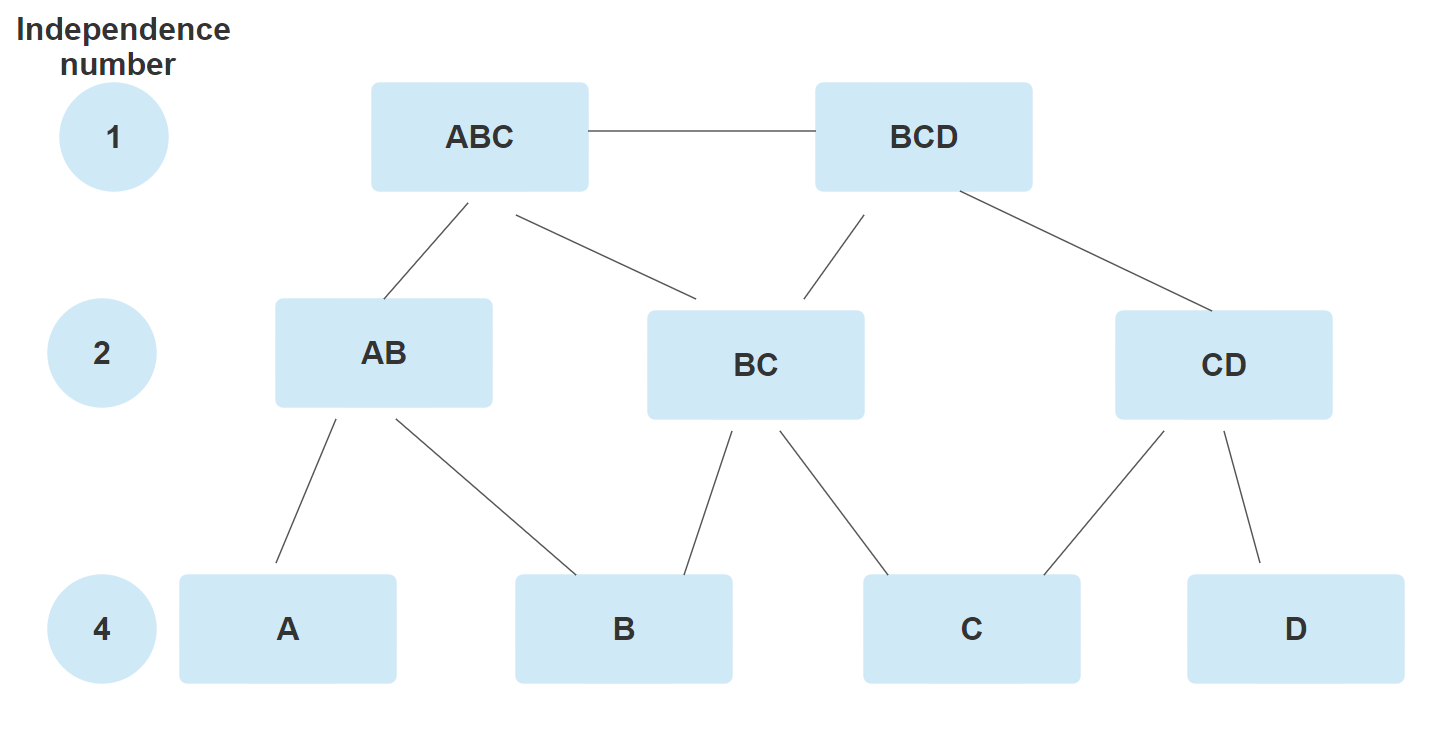
\includegraphics[width=0.7\textwidth]{Images/independence_graph.png}
    \caption{Example Independence Graph}
    \label{fig:exp_indp_graph}
\end{figure}

\bigbreak

In the cases when the other feasibility cuts still don't make the sub-problem feasible, a no good cut is added, which simply says at least one of the events turned on for period p must be turned off. It can be written as

\begin{equation}
    \sum_{\stackrel{e \in \E}{y_{e,p} = 1}}(1-y_{e, p}) \ge 1
\end{equation}

\subsubsection*{Optimality Cuts} \label{optimality}
If BSP has a non-zero objective value $M$, we need to add optimality cuts on the estimation variable $S2_p$. We make
the following observations:
\begin{itemize}
    \item Although we have access to the optimal solution to the sub-problem, it could be highly symmetric. Thus we
        are not able to reason about which specific events have contributed to the objective, rather we must consider
        which subsets of the events scheduled to the current time period that have caused the objective to be non-zero.
    \item The events which do not have undesired rooms can \emph{only} contribute to the feasibility of the sub-problem,
        not the optimality. To see this, suppose we have some optimal solution $x^*$ where removing an event $e_1$ with
        no undesired rooms from the current period would reduce the objective value. Then there exists an event $e_2$
        which is allocated to an undesired room in $x^*$ which can be allocated to the room which was occupied by $e_1$.
        But then we could have swapped the room allocations of $e_1$ and $e_2$ in $x^*$ to find a lower objective,
        violating our assumption of optimality.
\end{itemize}
 Therefore we need only consider those events which have undesired rooms, and because of the symmetry in the sub-problem,
 the strongest optimality cut we can make is one where the set $E_p \cap P2$ of events in the current period with
 undesired rooms is a subset of the events allocated:
\begin{equation}
    S2_p \geq M \left(1 - \sum_{e \in \E_p \cap P2} (1 - y_{e, p})\right)
\end{equation}

Furthermore, this cut is valid on $S2_{p'}$ for each $p' \in P$ with $R_{p'} \subseteq R_p$.



\end{document}